\ctitle{Definitions}

\paragraph{Convex programming}\index{Convex programming} Used to describe a special case of the general constrained optimization problem in which
%
\begin{itemize}[nolistsep,noitemsep]
    \item The objective function is convex
    \item The equality constraint functions $c_i(\cdot)$, $i \in \mathcal{E}$ are linear, and
    \item The inequality constraint functions$c_i(\cdot)$, $i \in \mathcal{I}$ are concave.
\end{itemize}

\paragraph{Convex function}\index{Convex function} The function $f$ is a \textit{convex function} if its domain $S$ is a convex set and if for any two points $x$ and $y$ in $S$, the following property is satisfied:
%
\begin{equation}
    f(\alpha x + (1 - \alpha)y) \leq \alpha f(x) + (1- \alpha) f(y), \quad \forall \alpha \in [0,1]
\end{equation}

\paragraph{Active set}\index{Active set} The active set $\mathcal{A}(x)$ at any feasible $x$ consists of the equality constraint indices from $\mathcal{E}$ together with the indices of the inequality constraints $i$ for which $c_i(x)=0$; that is
%
\begin{equation}
    \mathcal{A}(x) = \mathcal{E} \cup \{ i \in \mathcal{I} | c_i(x)=0 \}
\end{equation}

%\begin{comment}
LP:
%
\begin{equation}
    \mathcal{A}(x) = \{ i \in \mathcal{E} |  a_i^Tx=b_i\}\cup \{ i \in \mathcal{I} | x_i = 0 \}
\end{equation}

QP:
%
\begin{equation}
    \mathcal{A}(x) = \{ i \in \mathcal{E} \cup \mathcal{I} | a_i^Tx=b_i \}
\end{equation}
%\end{comment}

\paragraph{Basic feasible point}\index{Basic feasible point} A vector $x$ is a basic feasible point if it is feasible and if there exists a subset $\mathcal{B}$ of the index set $\{ 1, 2, \dots, n \}$ such that
%
\begin{itemize}[nolistsep,noitemsep]
    \item $\mathcal{B}$ contains exactly $m$ indices
    \item $i \notin \mathcal{B} \quad \Rightarrow \quad x_i = 0$ (that is, the bound $x_i \geq 0$ can be inactive only if $i \in \mathcal{B}$)
    \item The $m \times m$ matrix $\mathcal{B}$ defined by 
    \begin{equation}
        B = [A_i]_{i \in \mathcal{B}}
    \end{equation}
    is nonsingular, where $A_i$ is the $i$th column of $A$
\end{itemize}

\paragraph{Degeneracy}\index{Degeneracy} A basis $\mathcal{B}$ is said to be degenerate if $x_i = 0$ for some $i \in \mathcal{B}$, where $x$ is the basic feasible solution corresponding to $\mathcal{B}$. A linear program is said to be degenerate if it has at least one degenerate basis.

\paragraph{LICQ}\index{LICQ} (Linear Independence Constraint Qualification) Given the point $x$ and the active set $\mathcal{A}(x)$, we say that the LICQ holds if the set of active constraint gradients $\nabla c_i (x), \: i \in \mathcal{A}(x)$ is linearly independent.

\paragraph{Strict complementarity}\index{Strict complementarity} Given a local solution $x^*$ and a vector $\lambda^*$ satisfying the KKT conditions, we say that the strict complementarity condition holds if excactly one of $\lambda_i^*$ and $c_i(x^*)$ is zero for each index $i \in \mathcal{I}$. In other words, we have that $\lambda_i^* > 0$ for each $i \in \mathcal{I} \cap \mathcal{A} (x^*)$.

\paragraph{Search directions}\index{Search directions} Several approaches to line search directions can be used:

\hskip-0.5cm
\begin{tabularx}{\linewidth}{X X}
	\textbf{Method} & \textbf{Formula}\\
	\hline
	Steepest descent & $p_k=-\nabla f_k$\\
	Newton direction & $p_k^N=-(\nabla^2 f_k)^{-1}\nabla f_k$ \\
	Quasi-Newton direction & $p_k=-B_k^{-1}\nabla f_k$ \\
	\quad SR1(Symmetric-rank-one) & For updating $B_k$\\
	\quad BFGS & \\
	% Could add Conjugate gradient line
\end{tabularx}

\paragraph{The Wolfe conditions} \index{The Wolfe conditions}
Are used in line-search methods to decide if the decrease in the objective function is sufficient. The first one (\textit{sufficient decrease condition}):
\begin{equation}
    \label{eq:sufficient_decrease_condition}
    f(x_k+\alpha p_k) \leq f(x_k) + c_1 \alpha \nabla f_k^\top p_k
\end{equation}

There is also a second Wolfe condition (the \textit{curvature condition}: $\nabla f(x_k + \alpha_k p_k)^\top p_k \geq c_2 \nabla f_k^\top p_k$), but this condition can be dispensed if backtracking is used (find an acceptable step length by reducing $\alpha_k$ a finite number of trials -- it will eventually be small enough for \cref{eq:sufficient_decrease_condition} to hold).

\paragraph{Merit functions}\index{Merit functions} SQP methods often use merit functions to decide whether a trail step should be accepted. In line search methods, the merit function controls the size of the step.
%
\begin{equation}
    \begin{split}
        l_1\text{:} \quad \phi_1(x;\mu) &= f(x) + \mu \sum_{i \in \mathcal{E}} |c_i(x)| + \mu \sum_{i \in \mathcal{I}} [c_i(x)]^-\\
        %l_2\text{:} \quad \phi_2(x;\mu) &= f(x) + \mu || c(x) ||_2
    \end{split}
\end{equation}

Notation: $[z]^- = \text{max}\{0, -z\}$

The positive scalar $\mu$ is the penalty parameter, which determines the weight that we assigned to constraint satisfaction relative to minimization of the objective.

\textit{Exact merit function:} A merit function $\phi(x; \mu)$ is exact if there is a positive scalar $\mu^*$ such that for any $\mu > \mu^*$, any local solution of the nonlinear programming problem is a local minimizer of $\phi(x; \mu)$.

\paragraph{Maratos effect}\index{Maratos effect} The phenomenon where a merit function prevents rapid convergence because steps that make good progress toward a solution are rejected.
%
\begin{figure}[H]
	\centering
	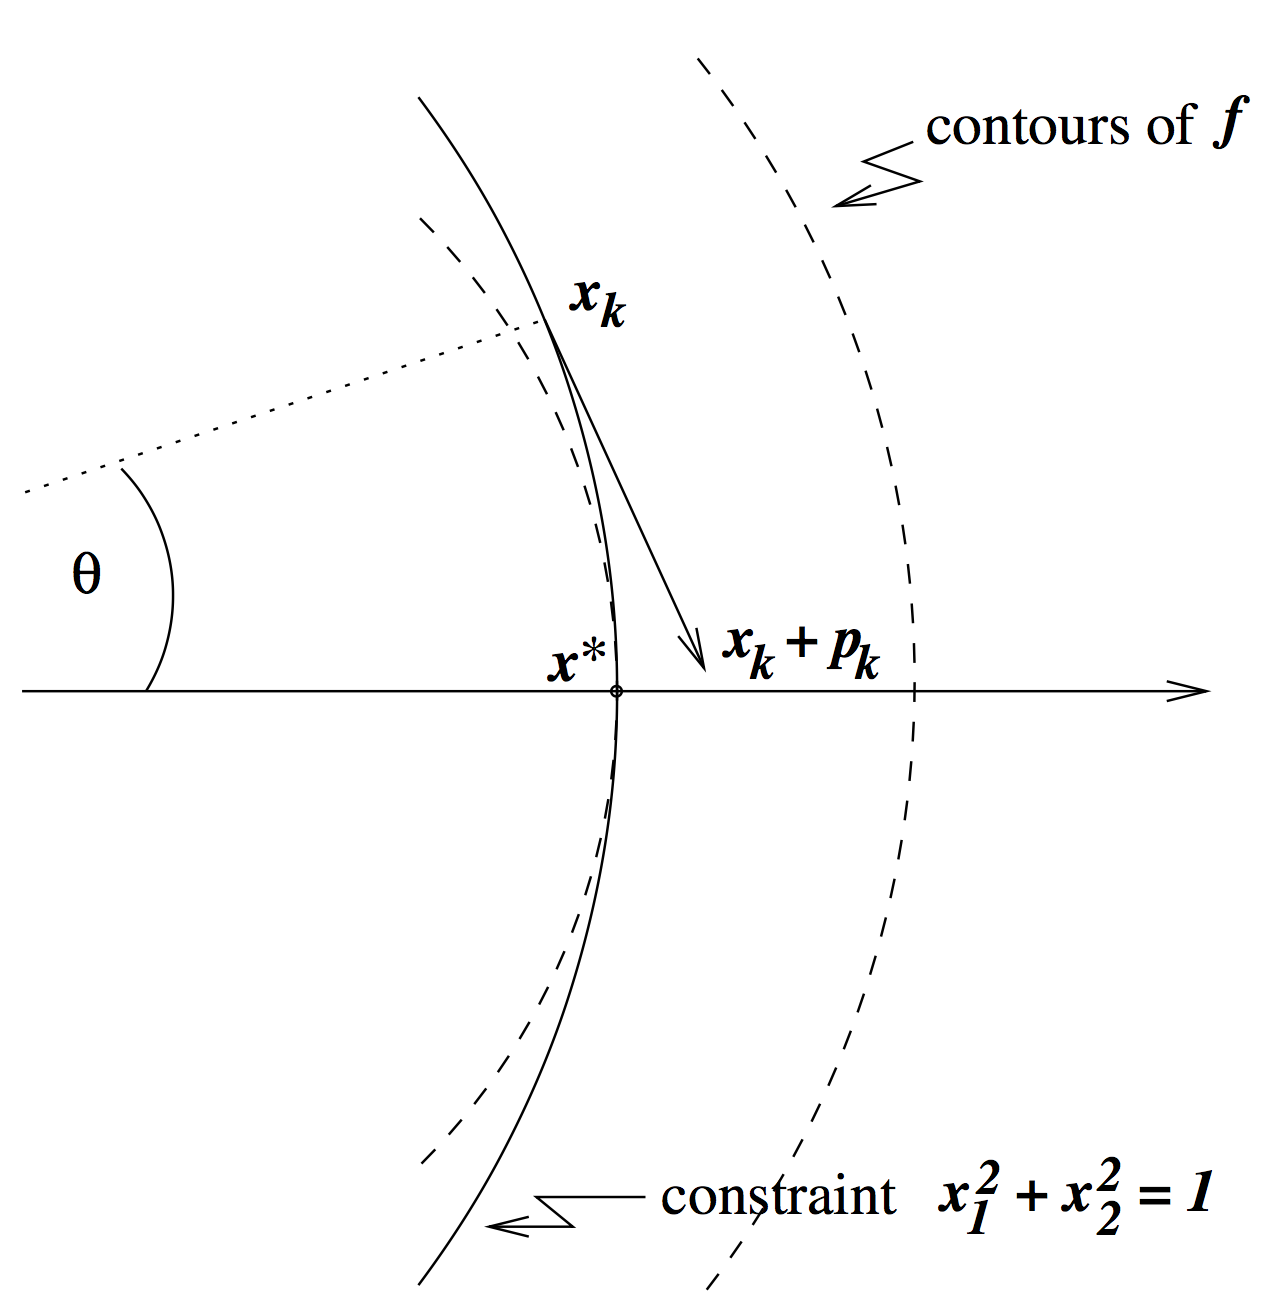
\includegraphics[width=0.3\textwidth]{images/maratos_effect}
	\caption{Maratos Effect}
	\label{fig:maratos_effect}
\end{figure}

% Definitions in course handout:
\paragraph{Model predictive control}\index{model predictive control} (MPC) A form of control in which the current control action is obtained by solving, at each sampling instant, a finite horizon open-loop optimal control problem, using the current state of the plant as the initial state; the optimization yields an optimal control sequence and the first control in this sequence is applied to the plant.
\begin{itemize}[nolistsep,noitemsep]
    \item Advantages
    \begin{itemize}[nolistsep,noitemsep]
        \item Inherent multivariable control
        \item Constraint handling, both on inputs and states
        \item The possibility of operation closer to constraints, usually leading to a more profitable process
        \item Understandable and intuitive theory
    \end{itemize}
    \item Challenges
    \begin{itemize}[nolistsep,noitemsep]
        \item Update model
        \item Tuned basic controllers
        \item Calibrated sensors
    \end{itemize}
\end{itemize}

\paragraph{Full-space VS Reduced-space formulation} \index{Full-space formulation} \index{Reduced-space formulation}
 \begin{itemize}[nolistsep,noitemsep]
     \item In full-space optimization, we include all inputs and all states in our objective function. The number of optimization variables is $\#\mathrm{steps} \cdot (\#\mathrm{states} + \#\mathrm{inputs})$.
     \item In reduced-space optimization, we remove the states from the objective function by replacing them using the model ($x_{t+1} = A_t x_t + B_t u_t$). The number of optimization variables is $\#\mathrm{steps} \cdot \#\mathrm{inputs}$.
 \end{itemize}

\hskip-0.5cm
\begin{tabularx}{\linewidth}{X X X}
	& \textbf{Pros} & \textbf{Cons}\\
	\hline
	\textbf{Full-space} & Often sparsity in matrices & Many variables\\
	\textbf{Reduced-space} & Less variables & Normally dense matrices
\end{tabularx}

\paragraph{Stabilizability}\index{Stabilizability} A system $(A,B)$ is stabilizable if all the uncontrollable modes are asymptotically stable.

\paragraph{Controllability}\index{Controllability} A system $(A,B)$ is controllable if for any initial state $x_0$ and any final state $x_N$, there exists a finite number of inputs $u_0, \dots, u_{N-1}$ to transfer $x_0$ to $x_N$.

\paragraph{Detectability}\index{Detectability}
A system $(A,D)$ is detectable if all the unobservable modes are asymptotically stable.

\paragraph{Observability}\index{Observability} A system $(A,D)$ is observable if the state $x_N$ can be determined from the system model, its inputs and outputs for a finite number of steps.

\paragraph{Linear quadratic Gaussian control} (LQG) The combination of an LQ controller and a Kalman filter.

\paragraph{Dual problem}\index{Dual problem}
The dual objective function $q: \mathbb{R}^n \rightarrow \mathbb{R}$ is defined as
%
\begin{equation}
    q(\lambda) \overset{\mathrm{def}}{=} \underset{x}{\mathrm{Inf}} \mathcal{L}(x, \lambda)
\end{equation}
%
The dual problem is defined as follows:
\begin{equation}
    \underset{\lambda \in \mathbb{R}^n}{\max} q(\lambda) \quad \text{subject to } \lambda \geq 0
\end{equation}